%%%%%%%%%%%%%%%%%%%%%%%%%%%%%%%%%%%%%%%%%%%%%%%%%%%%%%%%%%%%%%%%%%%%%%%%

%%% LaTeX Template for ECAI Papers 
%%% Prepared by Ulle Endriss (version 1.0 of 2023-12-10)

%%% To be used with the ECAI class file ecai.cls.
%%% You also will need a bibliography file (such as mybibfile.bib).

%%%%%%%%%%%%%%%%%%%%%%%%%%%%%%%%%%%%%%%%%%%%%%%%%%%%%%%%%%%%%%%%%%%%%%%%

%%% Start your document with the \documentclass{} command.
%%% Use the first variant for the camera-ready paper.
%%% Use the second variant for submission (for double-blind reviewing).

\documentclass{ecai} 
%\documentclass[doubleblind]{ecai} 

%%%%%%%%%%%%%%%%%%%%%%%%%%%%%%%%%%%%%%%%%%%%%%%%%%%%%%%%%%%%%%%%%%%%%%%%

%%% Load any packages you require here. 

\usepackage{latexsym}
\usepackage{amssymb}
\usepackage{amsmath}
\usepackage{amsthm}
\usepackage{booktabs}
\usepackage{enumitem}
\usepackage{graphicx}
\usepackage{color}

%%%%%%%%%%%%%%%%%%%%%%%%%%%%%%%%%%%%%%%%%%%%%%%%%%%%%%%%%%%%%%%%%%%%%%%%

%%% Define any theorem-like environments you require here.

\newtheorem{theorem}{Theorem}
\newtheorem{lemma}[theorem]{Lemma}
\newtheorem{corollary}[theorem]{Corollary}
\newtheorem{proposition}[theorem]{Proposition}
\newtheorem{fact}[theorem]{Fact}
\newtheorem{definition}{Definition}

%%%%%%%%%%%%%%%%%%%%%%%%%%%%%%%%%%%%%%%%%%%%%%%%%%%%%%%%%%%%%%%%%%%%%%%%

%%% Define any new commands you require here.

\newcommand{\BibTeX}{B\kern-.05em{\sc i\kern-.025em b}\kern-.08em\TeX}

%%%%%%%%%%%%%%%%%%%%%%%%%%%%%%%%%%%%%%%%%%%%%%%%%%%%%%%%%%%%%%%%%%%%%%%%

\begin{document}

%%%%%%%%%%%%%%%%%%%%%%%%%%%%%%%%%%%%%%%%%%%%%%%%%%%%%%%%%%%%%%%%%%%%%%%%

\begin{frontmatter}

%%% Use this command to specify your submission number.
%%% In doubleblind mode, it will be printed on the first page.

\paperid{123} 

%%% Use this command to specify the title of your paper.

\title{LLM-Augmented Optimization for Singapore Travel Itinerary Planning}

%%% Use this combinations of commands to specify all authors of your 
%%% paper. Use \fnms{} and \snm{} to indicate everyone's first names 
%%% and surname. This will help the publisher with indexing the 
%%% proceedings. Please use a reasonable approximation in case your 
%%% name does not neatly split into "first names" and "surname".
%%% Specifying your ORCID digital identifier is optional. 
%%% Use the \thanks{} command to indicate one or more corresponding 
%%% authors and their email address(es). If so desired, you can specify
%%% author contributions using the \footnote{} command.

\author[A]{\fnms{Daniel}~\snm{James}\orcid{....-....-....-....}\thanks{Corresponding Author. Email: danieljames.2023@mitb.smu.edu.sg.}}

\author[A]
{\fnms{Leonardo}\orcid{....-....-....-....}\thanks{Corresponding Author. Email: leonardo.2023@mitb.smu.edu.sg.}}

\author[A]
{\fnms{Jing Shen}~\snm{Tai}\orcid{....-....-....-....}\thanks{Corresponding Author. Email: js.tai.2023@mitb.smu.edu.sg.}}

\author[A]
{\fnms{Valerian}~\snm{Yap}\orcid{....-....-....-....}\thanks{Corresponding Author. Email: valerianyap.2023@mitb.smu.edu.sg.}}

\author[A]
{\fnms{Hoong Chuin}~\snm{Lau}\orcid{....-....-....-....}\thanks{Corresponding Author. Email: hclau@smu.edu.sg.}}

\address[A]{School of Computing and Information Systems, Singapore Management University}

%%% Use this environment to include an abstract of your paper.

\begin{abstract}
This paper presents a combined approach of Large Language Model (LLM) and Operation Research (OR) to develop an optimized travel planner for tourists visiting Singapore. Recognizing that traveler preferences vary significantly across demographics, we aim to generate customized itineraries that balance cost, travel time and personal satisfaction. We apply LLM agents to convert traveler's preferences in text format into a structured format that can be used for optimization. For optimization, we apply Adaptive Large Neighborhood Search (ALNS) with data enrichment techniques such as route matrix from Google Maps API to find out duration and price from point A to point B. Our contribution is the ability to make more-realistic itineraries, putting distance and cost into perspective, while focusing on traveler's best interest to minimize expenses and maximize satisfaction. We benchmarked against ... . Our approach ..., demonstrating the power of leveraging strengths of both LLM and ALNS in solving this problem.

\end{abstract}

\end{frontmatter}

%%%%%%%%%%%%%%%%%%%%%%%%%%%%%%%%%%%%%%%%%%%%%%%%%%%%%%%%%%%%%%%%%%%%%%%%

\section{Introduction}
The objective of this project is to develop a personalized travel itinerary planner for tourists visiting Singapore, capable of allowing natural language inputs and input fields into the demo product and generating a feasible yet personalized itinerary by minimizing travel cost, minimizing total transit time between locations, and maximizing satisfaction that aligns with Persona-specific preferences.

Our commercial inspiration was primarily drawn from Pelago by Singapore Airlines, an AI-powered trip planner platform that covers over 2,000 destinations. While Pelago appears to be employing an LLM-based recommendation engine, our work diverges by introducing a multi-agent LLM system that is combined with Operation Research (OR) optimization techniques.

Our goal in this paper includes answering the following questions: 
\begin{enumerate}
    \item Recognising the hallucination in LLM, to what extent can LLM alone generate realistic and feasible travel itineraries? Is Agentic AI needed to be used in our project?
    \item Assuming we have an LLM agent (e.g. a domain-expert in Singapore Attractions, equipped with memory, knowledge base and tools), can it handle reasoning consistency and personalisation without hallucinating? What is the trade-off for having multiple domain experts in our system?
    \item What are the quantitative and qualitative trade-offs between optimization-only, LLM-only, multi-agent, and hybrid optimization itinerary planning pipelines?
\end{enumerate}

This study is geographically and thematically scoped to the context of Singapore considering our familiarity of our local culture. Specifically, we focus on two categories of points of interest (POIs): (i) attractions, and hawker centres. In total, our curated dataset includes over 85 unique POIs.

%%%%%%%%%%%%%%%%%%%%%%%%%%%%%%%%%%%%%%%%%%%%%%%%%%%%%%%%%%%%%%%%%%%%%%%%

\section{Related Work}
Recent research highlights the growing synergy between LLMs and traditional optimization methods in itinerary planning.

For example, \textit{TRIP-PAL: Trip Planning with Guarantees by Combining LLMs and Automated Planners} (JP Morgan AI Research, 2024) explores how LLMs can be integrated with formal planning algorithms such as A* to produce reliable trip plans. This study shows that LLMs are capable of translating natural language inputs into structured formats compatible with optimization algorithms commonly used in operations research.

Similarly, \textit{Optimizing Travel Itineraries with AI Algorithms in a Microservices Architecture: Balancing Cost, Time, Preferences, and Sustainability} (Barua \& Kaiser, 2024) demonstrates how LLMs can support personalization within a modular microservices framework, enabling the coordination of multiple optimization objectives such as budget, travel time, user preferences, and sustainability.

\section{Problem Definition}
In this paper, we propose My Travel Itinerary Buddy – Automatic Itinerary (MITB – AI), where the goal is to generate multi-day travel itinerary for a tourist visiting Singapore, consisting of a sequence of POIs – including both attractions and hawker centres. This is also subjected to user-defined constraints (e.g. budget, number of days and person types) while optimizing for the following objectives: (1) minimize costs, (2) minimize travel time, and (3) maximize traveler’s satisfaction from online ratings. This problem can be classified as a multi-objective combinatorial optimization task, where the system must select and order POIs over multiple days while satisfying both hard and soft constraints (Fan, et al., 2024).

\subsection{Assumptions}
The assumptions that we have incorporated in our itinerary planners includes: 
\begin{itemize}
    \item all POIs are open from 9:00 AM to 10:00 PM.
    \item travelers return to the same hotel by the end of the day.
\end{itemize}

\subsection{Route Matrix Generation using Google Maps API}
To support accurate travel time estimation between POIs, we constructed a route matrix using Google Maps API.

\section{Contribution}
\textbf{!!! HELP THIS SECTION}.  Not to rely on outdated city census data
Domain expert view (pre-selection) not possible for large scale comparison and large n
since it is continuous, it is not possible to find by manual methods (scalable) and need a smart way of approximation
many applications

\section{Case Study}
TBA

\section{Proposed Approach}
\subsection{LLM and Multi-Agent Framework}
\textbf{!!! SHORTEN} Although LLMs are highly capable at interpreting and generating human-like text, they are passive systems—limited to single-turn type of interaction without persistent memory. This presents clear limitations when applied to travel itinerary planning, a task that requires structured decision-making, retrieval of external data (e.g., Google ratings, Cost of Attraction Entrance Fees), and context tracking across multiple steps. A passive LLM may generate a generic itinerary but lacks the capability to provide personalization such as “I prefer scenic routes” or “maximize shopping time within budget.”

To bridge this gap, we extend LLMs into autonomous agents by integrating three key capabilities: tool-calling (e.g., invoking Google Maps APIs), memory (to retain user goals and prior decisions), and Retrieval Augmented Generation (RAG) for incorporating external data into the reasoning process. This turns the LLM from a reactive text generator into a goal-driven planner capable of making informed decisions. Our system adopts this Agentic RAG architecture to retrieve attraction details, estimating hawker visit durations, and enrich itinerary planning with contextual knowledge beyond the LLM’s static knowledge from pre-training.

While a single agent can technically handle the entire itinerary pipeline, research has also shown that such monolithic setups often struggle with domain specialization. To address the limitation, we extend our architecture into a multi-agent framework where each agent focuses on a well-scoped domain task.

\begin{figure}[h]
    \centering
    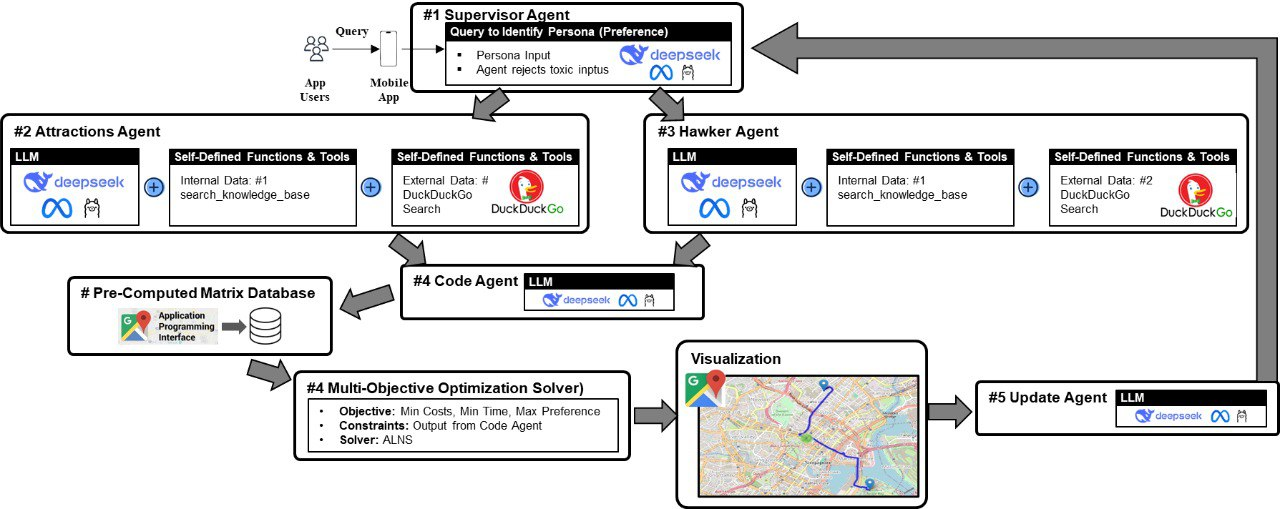
\includegraphics[width=1\linewidth]{6098288248590812104.jpg}
    \caption{Multi-Agent Architecture}
    \label{fig:Workflow Diagram}
\end{figure}

\subsection{Adaptive Large Neighborhood Search (ALNS)}
\textbf{!!! REPHRASE} ALNS is designed to solve optimization problems by iteratively destroying and repairing solutions. While traditional methods offer precise formulations, they struggle with scaling and flexibility in real-world data scenarios. In our project, ALNS was found to deal with our optimization problem better.

\section{Experimental Result}
TBA

\textbf{!!! try to use \url{https://arxiv.org/pdf/2402.01622} for the benchmark}
narratives:
1. agentic + alns is better than alns only and llm only
2. for feedback, compare 2B 2C 2D.
    - ideally: 2d is best, but slowest

\section{Conclusion}
TBA

% For instructions on how to submit your work to ECAI and on matters such 
% as page limits or referring to supplementary material, please consult 
% the Call for Papers of the next edition of the conference. Keep in mind
% that you must use the \texttt{doubleblind} option for submission. 


% You presumably are already familiar with the use of \LaTeX. But let 
% us still have a quick look at how to typeset a simple equation: 
% %
% \begin{eqnarray}\label{eq:vcg}
% p_i(\boldsymbol{\hat{v}}) & = &
% \sum_{j \neq i} \hat{v}_j(f(\boldsymbol{\hat{v}}_{-i})) - 
% \sum_{j \neq i} \hat{v}_j(f(\boldsymbol{\hat{v}})) 
% \end{eqnarray}
% %
% Use the usual combination of \verb|\label{}| and \verb|\ref{}| to 
% refer to numbered equations, such as Equation~(\ref{eq:vcg}). 
% Next, a theorem: 

% \begin{theorem}[Fermat, 1637]\label{thm:fermat}
% No triple $(a,b,c)$ of natural numbers satisfies the equation 
% $a^n + b^n = c^n$ for any natural number $n > 2$.
% \end{theorem}

% \begin{proof}
% A full proof can be found in the supplementary material.
% \end{proof}

% Table captions should be centred \emph{above} the table, while figure 
% captions should be centred \emph{below} the figure.\footnote{Footnotes
% should be placed \emph{after} punctuation marks (such as full stops).}
 
% \begin{table}[h]
% \caption{Locations of selected conference editions.}
% \centering
% \begin{tabular}{ll@{\hspace{8mm}}ll} 
% \toprule
% AISB-1980 & Amsterdam & ECAI-1990 & Stockholm \\
% ECAI-2000 & Berlin & ECAI-2010 & Lisbon \\
% ECAI-2020 & \multicolumn{3}{l}{Santiago de Compostela (online)} \\
% \bottomrule
% \end{tabular}
% \end{table}

%%%%%%%%%%%%%%%%%%%%%%%%%%%%%%%%%%%%%%%%%%%%%%%%%%%%%%%%%%%%%%%%%%%%%%%%


%%% Use this command to include your bibliography file.

\bibliography{mybibfile}

\end{document}
%%%%%%%%%%%%%%%%%%%%%%%%%%%%%%%%%%%%%%%%%%%%%%%%%%%%%%%%%%%%%%%%%%%%%%

Sure, here are the key pointers and follow-ups from the meeting:

Initial site selection using community centroids:


Concern that naively selecting community centroids as candidate sites without considering competitor and allied stores may miss out on potentially better nearby locations.
Suggestion to shift centroids away from competitors and towards population concentrations for better capture.
Explore metrics like silhouette index that consider cohesion to population and separation from competitors.


Varying community granularity:


Instead of fixing community sizes, explore varying the granularity - make communities smaller or larger.
This allows searching a larger solution space and potentially finding better centroids/sites.
Relates to the idea of making the discrete approach tend towards a continuous solution space.


Two-level site selection:


First select top sites within each micro-community/smaller granularity.
Then combine these top micro-sites as candidates for the overall macro-community selection.


Comparison with continuous approach:


A major contribution could be showing the discrete community approach performs comparably to a continuous approach, but with much higher computational efficiency.
This requires implementing and comparing against a true continuous baseline.


Clarify terminology:


Need to clearly define and distinguish between "solution neighborhood", "search space", etc. in the paper.
Response required to the reviewer's comment seeking clarification on these terms.


Rework/strengthen contributions:


Some concerns that the stated contributions (discrete to continuous, eliminating human bias, generalizability) may not be very strong.
Need to rethink and articulate the real novel contributions more convincingly.


Literature review:


Review recent literature to identify relevant work still using static/non-dynamic models to better justify this approach.


Meeting with Proflow:


Proflow wants to see the full paper draft before the next meeting, likely early next week.
Kar Way may not be available tomorrow due to his daughter's school event.

Overall, there are suggestions to improve the site selection process, explore varying granularities, compare against a continuous baseline, clarify terminology, rework the contributions, review recent literature, and prepare for the next meeting with the full draft.
